\documentclass{standalone}
\usepackage{tikz}
\usetikzlibrary{arrows,positioning,decorations.pathreplacing} 
\tikzset{
    %Define standard arrow tip
    >=stealth',
    %Define style for boxes
    point/.style={
           rectangle,
           rounded corners,
           draw=black, very thick,
           text width=6em,
           minimum height=2em,
           font=\sffamily,
           text centered},
    annote/.style={
          font=\sffamily
    },
    % Define arrow style
    arrow/.style={
           ->,
           thick,
           shorten <=2pt,
           shorten >=2pt,},   
}
\begin{document}
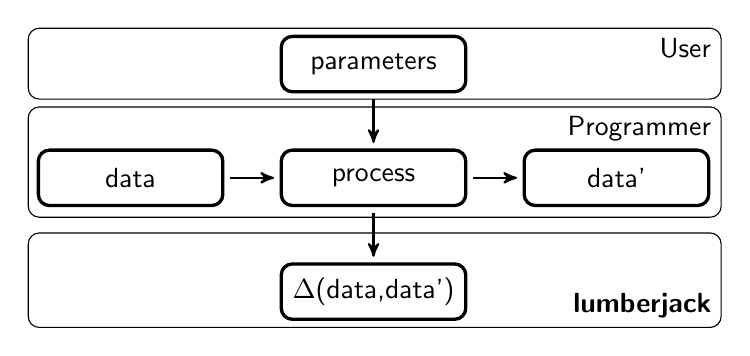
\begin{tikzpicture}
  \node[point] (in) {data};
  \node[point, right=7mm of in]  (mod){process};
  \node[point, right=7mm of mod] (out){data'};
  \node[point, above=7mm of mod] (par){parameters};
  \node[point, below=7mm of mod] (log){$\Delta$(data,data')};
\draw [rounded corners] (-1.3,1.0) rectangle ++(8.8,0.9) 
      node [anchor=north east] {\textsf{User}};

\draw [rounded corners] (-1.3,-0.5) rectangle ++(8.8,1.4) 
      node [anchor=north east] {\textsf{Programmer}};

\draw [rounded corners] (-1.3,-0.7) rectangle ++(8.8,-1.2) 
      node [anchor=south east] {\textbf{\textsf{lumberjack}}};
  \path (in.east) edge[arrow] (mod.west);
  \path (mod.east) edge[arrow] (out.west);
  \path (par.south) edge[arrow] (mod.north);
  \path (mod.south) edge[arrow] (log.north);
\end{tikzpicture}
\end{document}
